\documentclass{article}

% if you need to pass options to natbib, use, e.g.:
% \PassOptionsToPackage{numbers, compress}{natbib}
% before loading nips_2016
%
% to avoid loading the natbib package, add option nonatbib:
% \usepackage[nonatbib]{nips_2016}

%\usepackage{nips_2016}

% to compile a camera-ready version, add the [final] option, e.g.:
% \usepackage[final]{nips_2016}

\usepackage[utf8]{inputenc} % allow utf-8 input
\usepackage[T1]{fontenc}    % use 8-bit T1 fonts
\usepackage{hyperref}       % hyperlinks
\usepackage{url}            % simple URL typesetting
\usepackage{booktabs}       % professional-quality tables
\usepackage{amsfonts}       % blackboard math symbols
\usepackage{nicefrac}       % compact symbols for 1/2, etc.
\usepackage{microtype}      % microtypography
\usepackage{natbib}
\usepackage{graphicx}
\usepackage{subfigure}
\usepackage{algorithm}
\usepackage{algorithmic}
\usepackage{color, soul}

\title{Ensemble Based Neural Network for the Classification of MURA Dataset }
\usepackage[final]{nips_2016}

% The \author macro works with any number of authors. There are two
% commands used to separate the names and addresses of multiple
% authors: \And and \AND.
%
% Using \And between authors leaves it to LaTeX to determine where to
% break the lines. Using \AND forces a line break at that point. So,
% if LaTeX puts 3 of 4 authors names on the first line, and the last
% on the second line, try using \AND instead of \And before the third
% author name.

\author{
  Mithun Ghosh\\
  Department of \\
 Systems \& Industrial Engineering\\
  University of Arizona\\
  Tucson, AZ 85719 \\
  \texttt{mithunghosh@email.arizona.edu} }
  %% examples of more authors
  
  %% \AND
  %% Coauthor \\
  %% Affiliation \\
  %% Address \\
  %% \texttt{email} \\
  %% \And
  %% Coauthor \\
  %% Affiliation \\
  %% Address \\
  %% \texttt{email} \\
  %% \And
  %% Coauthor \\
  %% Affiliation \\
  %% Address \\
  %% \texttt{email} \\
%%}

\begin{document}
 

\maketitle

\begin{abstract}
  Musculoskeletal Radiographs (MURA) dataset, proposed by Stamford Machine Learning (ML) group, contains 40,561 images of bone X-rays from 14,863 studies.
  %These images are labeled manually by radiologists as two classes: normal and abnormal. Also, these images are taken from seven areas of the human body: Wrist, Elbow, Finger, Humerus, Forearm, Hand, and Shoulder. Normal indicates the bones in a specific region are not broken or damaged while abnormal means something is not right in that bones.
  The X-ray images belong to seven body areas of upper extremity- Wrist, Elbow, Finger, Humerus, Forearm, Hand, and Shoulder. The data are classified manually by radiologists into two classes- normal or abnormal. 
  %The dataset further contains 207 musculoskeletal studies as test data 
  These data samples are labeled using majority vote by six board-certified Stanford radiologists. The majority votes of these radiologists' labels are considered as gold standard.
  The presence of such rich,complex and diverse labeled dataset inspires to build an accurate but simpler model for bone anomaly detection. 
  %In order to increase the detection capability of the model and to get an estimate of the radiologist performance, additional test data are the label from six board-certified Stanford radiologists which consists of 207 musculoskeletal studies.
  %Majority vote of a group of three radiologists serves as the gold standard on these test sets.
  The model proposed by Stamford ML group is a 169 layer deep computationally complex Neural Network (NN), that requires a Graphical Processing Unit (GPU) for implementation. This leads to the necessity of smaller neural network based model that are executable on general purpose computers. Moreover, the 169 layer deep model works well on par with the gold standard except for the humerus radiographs, despite the presence of humerus data labeled with high accuracy.
  Therefore, in this work we propose an ensemble of smaller neural networks and convolution neural network for highly accurate classification of MURA study images of humerus. We use Adaboost algorithm to train this model. The performance of this model is evaluated using training error, validation error, and Cohen's kappa coefficients. The model is available at \url{https://github.com/mythgotham007/Mura_Humerus_CNN-NN/import} .
  %In this paper, we present an ensemble focus on the Humerus radiographs of MURA data to improve the accuracy of these data with efficiency. We use an ensemble of a neural network to improve the accuracy and kappa value in the model.
\end{abstract}

\section{Introduction}
The current era of big data has accelerated the development of machine learning based models. It is becoming increasingly crucial that these models can handle large dataset without losing any significant information. Out of the several application fields of these models, the medical sector is one of the most demanding sectors. It requires models that can classify large amount of data with high accuracy. Among the several machine learning approaches, neural network is in its prime to handle large dataset~(\cite{deng}) with significant accuracy. This makes it a suitable choice for medical applications.

There are several branches in medical field where classification models can play an important role. The radiographic study is one such branch, where the correct classification of studied data is of utmost importance. According to WHO (World Health Organization), musculoskeletal conditions are becoming a major burden on individuals.~\cite{woolf_03} discussed the burden of the major musculoskeletal conditions. About 1.7 billion people are affected by this conditions worldwide. Based on the classification outcome, the patient may need to go further diagnosis and treatment. But most of the time it is not easy even for the naked eye to detect any abnormality in the X-ray images which we can notice in some of the images from Fig.~\ref{xray}. Mistreatment due to the misclassification is thus critical in any situation for that patient.

MURA is a large dataset of musculoskeletal radiographs recently proposed by Stamford Machine Learning (ML) group. This dataset can help train and create accurate models for classification in radiographic studies. It contains 14,863 studies with 40,561 images. Each study in the data contains multiple views of the targeted body part, which are labeled by radiographers as normal or abnormal. These are high resolution images that make the size of the whole dataset around 3.3 GB. The large size of this dataset and the crucial accuracy requirements of the radiographic study sector requires neural network based approaches.
\begin{figure}[t]
\centering
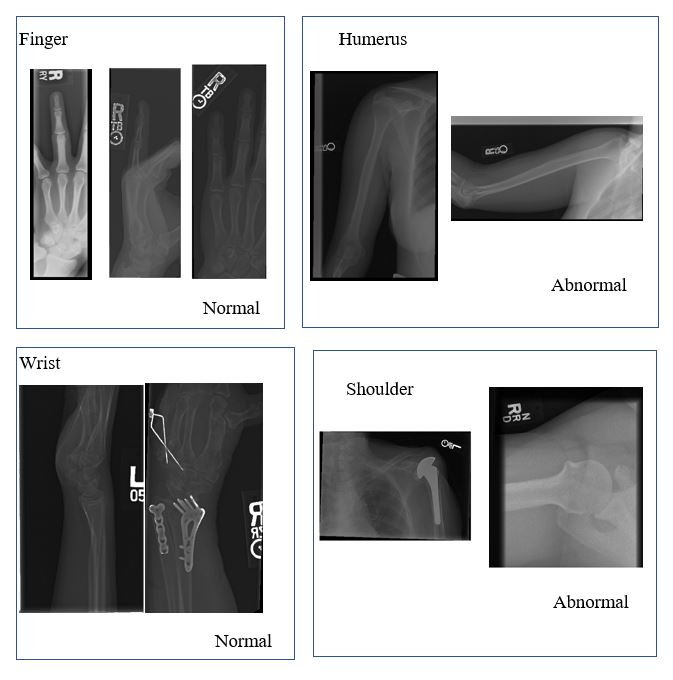
\includegraphics[width=0.6\textwidth]{xray.JPG}
\caption{MURA dataset contains 14863 images of the radiography of musculoskeletal studies of the upper extremity. In each of the study multiple views are manually labeled by radiologists. Right side of the above Figure explains some normally labeled images of Elbow and Wrist, respectively wherein left side describes some abnormal images from the Humerus and Shoulder, respectively.}
\label{xray}
\end{figure} 

The Stamford ML group proposed a 169 layer deep neural network model of dense layers to reliably classify the MURA dataset. This model classifies most of the X-ray images of different body parts with high degree of agreement with the radiologist classifiers (gold standard). However, it shows low agreement with gold standard for finger and humerus dataset. In case of the finger dataset,~\cite{pranav_18} shows that the existing finger dataset labels had low value of Cohen's kappa coefficient. This causes the model to perform poorly. However, for humerus data, despite presence of highly accurate labels the model performs poorly. Moreover, the computational complexity of this deep neural network model requires a GPU to execute. In order to address these two issues, this work presents an ensemble model of 12 layered neural networks. This model can run on a general purpose computer without the necessity of a GPU. But to get the full advantage of the model, we require some high performing computer(HPC) due to the large size of the image. We also build an autoencoder with Convolution Neural Network(CNN). The testing and training has been carried out on humerus dataset only.

The following part of this paper is organized as- section 2 describes the details of MURA dataset, section 3 describes the proposed ensemble model, section 4 contains the model interpretation, section 5 compares the performance of the proposed model with Stamford ML group's model,  section 6 describes the related works and section 7 discusses the overall findings.
%Therefore, the classification of large sized MURA dataset requires neural network based approaches.  Some of the samples of the dataset are given below for illustration.\\
%\textbf{FIG}\\
%The Importance of correctly classify in radiographic study is utmost important. Based on the classification, the patience may need to go further diagnosis and treatment. But most of the time it is not so easy ever in naked eye to detect any abnormality in the X-ray images which we can see some of the images from Figure 1. Mistreatment due to the misclassification is thus critical in any situation for that patience. According to WHO (World Health Organization), musculoskeletal conditions are becoming a major burden on individuals. ~\cite{woolf_03} discussed the burden of the major musculoskeletal conditions. About 1.7 billion people are affected by this conditions worldwide. Musculoskeletal conditions are the most common cause of severe long term pain and physical disability. Millions of people are suffering from these pain. Roughly 30 percent of American adults are presently impacted by joint pain, inflammation, or motion limitation [3]. Musculoskeletal circumstances are a diversified group in terms of psychopathology but are related anatomically and by their connection with discomfort and deficient cognitive function. They include a spectrum of situations varying from severe earliest stages and low-lived to longtime abnormalities, including osteoarthritis, rheumatoid arthritis, osteoporosis, and low back pain. The proliferation of many of these situations increases significantly with age, and many have been impacted by variables of way of life, such as obesity and lack of exercise. The increasing number of elderly people and the global changes in lifestyle imply that the burden on people and society will rise dramatically. This was recognized by the United Nations and the WHO with their endorsement. The burden of autonomic dysfunction can be measured in units of the difficulties associated with them, i.e. the pain or deficient operating (disability) linked to the musculoskeletal system, or in relation to the cause, such as joint illness or trauma. The burden should also be deemed as to who is at danger. A study of available data as aspect of the Bone and Joint Monitor Venture in co-operation.
\begin{figure*}[t]
\subfigure{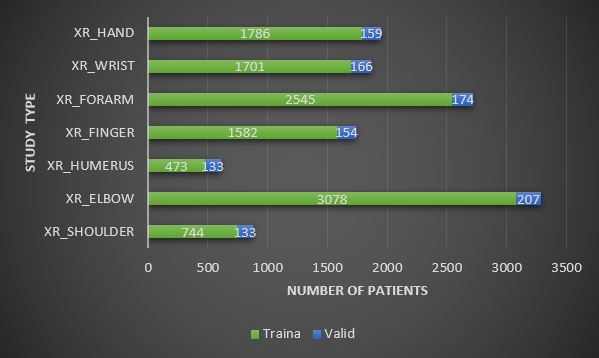
\includegraphics[width=0.44\textwidth]{std.JPG}}
\hspace{0.1\textwidth}
\subfigure{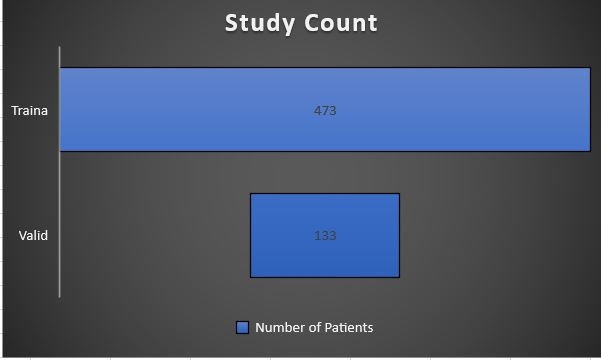
\includegraphics[width=0.44\textwidth]{stdhum.JPG}}
\caption{Left: Statistics of the data in each of the seven categories of the studies. In train set XR\_WRIST has maximum number of patients, followed by XR\_FINGER, XR\_HUMERUS, XR\_SHOULDER, XR\_HAND, XR\_ELBOW and XR\_FOREARM. X\_FOREARM with 606 patients has got the least number. Similar pattern can be seen in valid set, XR\_WRIST has the maximum, followed by XR\_FINGER, XR\_SHOULDER, XR\_HUMEROUS, XR\_HAND, XR\_ELBOW, XR\_FOREARM. Here XR\_FINGER defines radiographs of  Finger upper extremity. Right: Data Statistics for Humerus Data}
\label{distribution}
\end{figure*}

\section{MURA}
The task in MURA dataset is to find the binary class of $\{0,1\}$. Each study contains one or more views of images and the expected output is then denoted as 0 or 1. We denote 0 as normal and 1 as abnormal. A brief summary of the study data is given below:\\
In the official MURA dataset website (\url{https://stanfordmlgroup.github.io/competitions/mura/}) we can see the performance of various authors model in different categories. Some of these model perform well for different categories. But For upper extremity categories: Humerus and Finger, almost all of the models perform worst. This may be due to the fact that, the images in these categories are not so clear. Also, the number of samples are not sufficiently high in these categories. We can look that in right side of Fig.~\ref{xray}, these images are not so clear to be easily classified by the models. Thus, for this reason, we concentrate our model to the Humerus cases. In left side of Fig.~\ref{distribution}, we can also see that number of studied patients are very few for both training and test dataset in Humerus study.

\subsection{Data Collection}
Data is collected from MURA dataset official website. A large number of patients are studied with multiple view of their radiographs.  Total number of radiographs image is 14,863 that was collected from 12,713 patients with a total of 40,561 multi-view  X-ray images. These images belong to one of the seven standard upper extremity radiographic study types as described previously.\\
At the moment of medical radiographic analysis in the diagnostic radiology atmosphere between 2001 and 2012, each study was manually marked as normal or abnormal by Stanford Hospital board-certified radiologists. The labeling was conducted during the assessment of DICOM(Digital Imaging and Communications in Medicine) images on a medical grade display of at least 3 megapixels {PACS}(Picture Archiving and Communication System) with max luminance of 400 $cd/m^2$ and min luminance 1 $cd/m^2$ with pixel size of 0.2 and native resolution of 1500 x 2000 pixels. Clinical images vary in pixel density and aspect proportions. The data set is divided into training sets (11,184 patients, 13,457 studies, 36,808 images), validation sets (783 patients, 1,199 studies, 3,197 images), and test sets (206 patients, 207 studies, 556 images). There is no crossover between any sets in patients.

\subsection{Test Set Collection}
Extra labels of data are obtained from board-certified Stanford radiologists on the test set, composed of 207 musculoskeletal experiments, to assess models to get a resilient assessment of radiologist performance. The radiologists individually examined and categorized each study in the test set as a DICOM  file as normal or abnormal in the clinical reading room environment using the {PACS}. Radiologists have an average of 8.83 years of professional experience varying from 2 to 25 years. The radiologists had no direct exposure to any clinical data. Classifications have been entered into a standardized data entry program.

\subsection{Abnormality Analysis}
In order to investigate the types of abnormalities present in the dataset, we reviewed the radiologist reports
to manually label 100 abnormal studies with the abnormality finding: 53 studies were labeled with fractures, 48 with hardware, 35 with degenerative joint diseases, and 29 with other  abnormalities including lesions and subluxations. 

\section{Model}
%The proposed model in this paper uses an ensemble technique with smaller deep neural networks to perform classification. In other related works, usually a very deep neural network with large amount of nodes are incorporated into the model to classify the MURA dataset. For example, ~\cite{pranav_18} considered 169 layers deep neural network to achieve a good results. This takes a lot of computational resources. So, our aim is to take advantage of ensemble techniques to alleviate resource deficiency. We use adaboost or adaptive boosting techniques of ensemble learning in neural network. ~\cite{pranav_18} and other authors, got high accuracies in most of the upper extremities except Humerus and Finger. That’s why we mainly focus on one of them : Humerus. We use ========(neural structure)==================================.\\
The proposed ensemble model is made up of smaller deep neural networks. These neural networks are trained on the train data from humerus X-ray images of MURA using the Adaboost algorithm~(\cite{adaboost}). Section 3.1 explains the structures and training of each of these smaller neural networks. Section 3.2 explains the overall ensemble training and prediction methods.

\subsection{Network Architecture and Training}
The structural details of each smaller deep neural networks is shown in Fig.~\ref{nn_struct}. Each neural network has 10000 nodes in input layers and one node in output layer. There are 10 hidden layers between input and output layer. As the network grows deeper, number of nodes into each new layer reduces. These neural networks are modeled using models available in Keras library.\\
Now, The structural details of each of CNN is shown in Fig.~\ref{rgbo}. Each of the CNN consists of kernel window size of 4x4 with stride one and Maxpooling of 2x2. This auto-encoder network compress the size of the image to from 100x100 to 9x9 with minimum reconstruction error. After that, the layers are flatten and fully connected to dense layer with 500 nodes and rectified linear activation function and then another dense layer with 20 nodes and finally the two output layer. 

\begin{figure}
    \centering
    \includegraphics[width=0.8\linewidth]{nnstruct.jpg}
    \caption{Structure of the small neural network used as weak classifier in the ensemble model.}
    \label{nn_struct}
\end{figure}
\begin{figure}
    \centering
    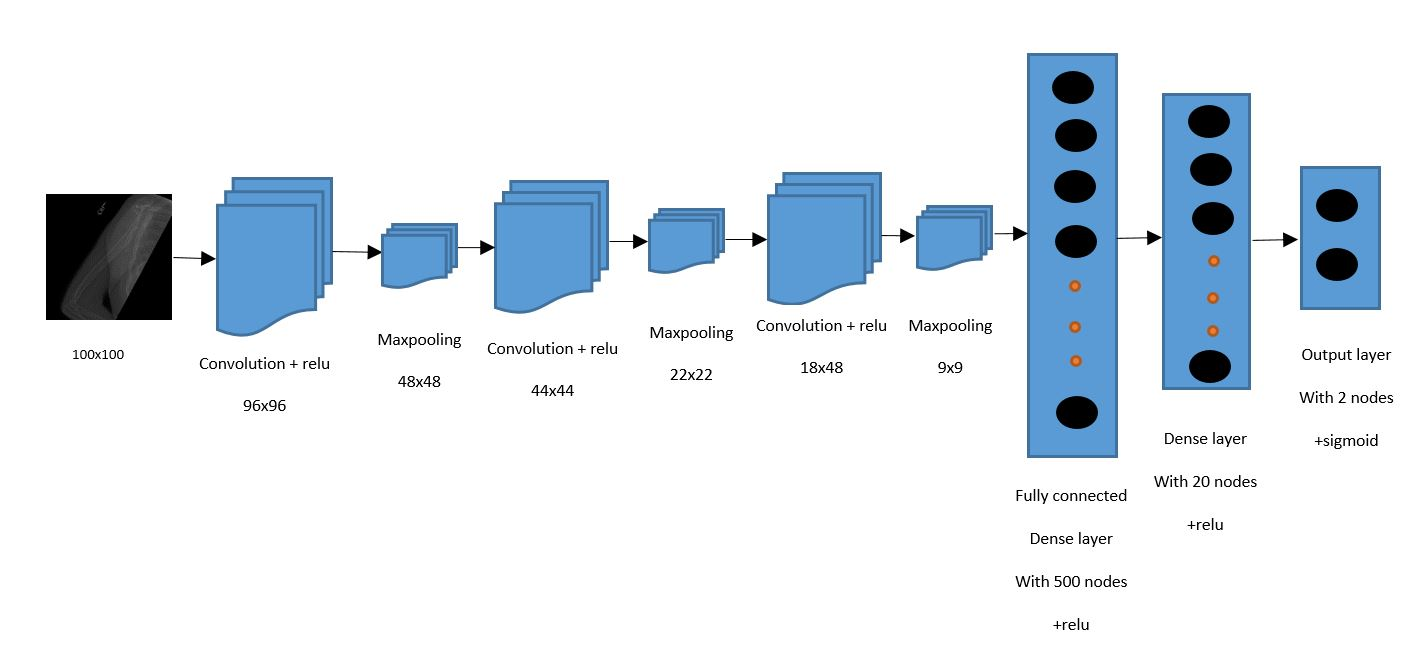
\includegraphics[width=1\linewidth]{rgbo1.JPG}
    \caption{Structure of the small convolution neural network used as weak classifier in the ensemble model.}
    \label{rgbo}
\end{figure}
In order to optimize the network, each neural network uses the ADADELTA optimizer~(\cite{adadelta}), a novel per-dimension learning rate method for gradient descent. The method does not require any  manual tuning of a learning rate and appears robust to noisy gradient information, different model architecture choices, various data modalities and selection of hyperparameters. We considered minimizing the binary cross entropy loss as there are only two output classes- Normal and Abnormal. For image $X$ of study type $T$ in the training set, the loss is:
\begin{equation}
    L(X,y) = w_{T,1}y \log{p(Y=1|X)} - w_{T,0}(1-y) \log{p(Y=0|X)}.
\end{equation}
Here, $y$ and $p(Y=i|X)$ is the label and probability that the network assigns to the label $i$, respectively. Also, $w_{T,1} = \frac{|N_T|}{|A_T|+|N_T|}$ and $w_{T,0} = \frac{|A_T|}{|A_T|+|N_T|}$, where $N_T$ and $A_T$ defines normal and abnormal images of the particular study $T$ in the training set, respectively.

The hidden layer nodes used Rectified Linear Units (ReLU) function as activation function. This activation function is easier to calculate and enables faster convergence during training. The output layer uses Sigmoid function for activation. The threshold for the output node is set at 0.5. The ReLU and Sigmoid functions are shown in equation~\ref{relu} and~\ref{sigm} respectively.

\begin{equation}
    f(x)=\max(0,x)
    \label{relu}
\end{equation}

\begin{equation}
    \sigma(x)=\frac{1}{1+e^{-x}}
    \label{sigm}
\end{equation}

Among the several training parameters of the neural networks, we kept the training epoch number as a variable to study the effect of epochs on the classifiers performance on training and validation dataset. There are overall 1272 training images on humerus. The batch size is kept 30 during training. We vary the epoch sizes from 10 to 40.
%=======DATA normalization and Preprocessing================\\
%=======Weight update, optimization method used,batch epoch,=======\\

%The structural details of these neural networks are shown in~\ref{nn_struct}. Each neural network has 10000 nodes in input layers and 1 node in output layer. The MURA images are cropped to $100\times100$ pixels
%Adaboost algorithms are described below:\\
%\textbf{Algorithm}\\
%Hypothesis h in our case is neural network. The final output which is hypothesis H is taken from simply linear combination of the decision on a sample. 

\subsection{Ensemble Training and Prediction}
In the previous sections, the smaller neural networks are described. Each of these neural networks perform slightly better than a random classifier on the humerus training data. Therefore, we use the Sampling based Adaboost algorithm to train these neural networks with emphasis on the wrong classifications made by previously trained classifier. The ensemble model contains 5 small neural networks, which implies that 5 Adaboost iterations are used to train the model. For the CNN, due to lack of resource we just fitted it with five classifiers and ten epoches. 

The overall flow of the ensemble training is shown in Algorithm~\ref{alg1}. Initially, all the training images and their labels are imported from directories. The training images contain different amount of pixels. We resize all the images into $100\times100$ pixels, and flatten it to $1\times10000$ pixels shape. After that, we normalize these pixel values between $[0,1]$. Therefore we launch the iterative training following Adaboost algorithm, with the initial training data distribution ($D$) equal for each sample. In each iteration, a small NN or CNN is trained on training data sampled as per the updated distribution by the previous iteration. Upon completion of training, the weighted error $\epsilon_t$ is calculated (step 5). Based on $\epsilon_t$, the weight of the trained neural network, $\alpha_t$ is calculated (step 6). Then, the distribution $D$ is updated as per the equation described in step 7 of the algorithm. Here, $Z_t$ is a normalization term. Finally, the training dataset is sampled as per the updated $D$ for training purposes in the next iteration.

\begin{algorithm}[t]
    \caption{Training steps for neural network ensemble model using Adaboost Algorithm}
    \label{alg1}
\begin{algorithmic}[1]
    \STATE \textbf{Input:} $S:={\{x_i,y_i\}}_{i=1}^N$,    \textit{Learning rounds $T$}, and \textit{hypothesis class $H$}\\
    \STATE \textbf{Initialize:} \textit{Distribution $D_1(i)=\frac{1}{n}$}, $S:=normalize(S)$\\
    \FOR {$t=1,2,....,T$}
    \STATE $h_t=arg min_{h\in{H}}\hat{err}(h,S,D_t)$
    \STATE $\epsilon_t=\sum{D_t(i)[h(x_i)\neq{y_i}]}$
    \STATE $\alpha_t=\frac{1}{2}log(\frac{1-\epsilon_t}{\epsilon_t})$
    \STATE $D_{t+1}(i)=\frac{D_t(i)}{Z_t}exp(-\alpha_ty_ih_t(x_i))$
    \ENDFOR
\end{algorithmic}
\end{algorithm}
The prediction using this ensemble neural network model is conducted as per the following equation.
\begin{equation}    
H(x)=sign(\sum_{t=1}^T\alpha_th_t(x))
\label{ensemble_predict}
\end{equation}
    

\section{Model Interpretation}
As mentioned before, we aim to focus on the most vulnerable upper extremity in MURA dataset namely, Humerus. We calculated both training error and testing error based on train and test data. The error calculation formula:
\begin{equation}
    Error=\frac{\sum_{i=1}^n(y_i-\hat{y_i})}{n}
\end{equation}

where $y_i$ defines the $i$th true observed value , $\hat{y_i}$ defines corresponding predicted value form our model and $n$ defines length of the observation. 

The kappa coefficient ($\kappa$) of Cohen is a measurable statistic of inter-rater agreement for qualitative (categorical) items. It is generally regarded to be a much more robust measure than a simple percentage agreement calculation, as the probability of the arrangement occurring by chance is taken into consideration by $\kappa$. The kappa of Cohen measures the agreement between two raters, each classifying $N$ items into categories that are mutually exclusive. \cite{galton} is ascribed to the first mention of a kappa-like statistics. ${\kappa }$ is defined as:
\begin{equation}
\kappa=\frac{p_o-p_e}{1-p_e}    
\end{equation}
where $p_o$ is the relative observed agreement among raters and $p_e$ is the hypothetical chance agreement probability, using the observed data to calculate the probabilities of each observer seeing each category randomly.  If the raters are in full agreement, $\kappa=1$. If the raters do not agree other than what is expected by chance (as given by $p_e$), $\kappa=0$ , which implies that there is no effective agreement between the two raters or the agreement is worse than random. In the following section, we describe our model performance using these statistics. 

\section{Radiologist vs Model Performance}
In order to evaluate the performance of our proposed model, we use training error, validation error, and Cohen's kappa coefficient ($\kappa$) for both training and validation data. Table~\ref{results} presents the $\kappa$ values of classifications made by the Radiologist with best performance, model by Stamford ML group, and model proposed in this work. The results contain model performance for different training epochs. All the mentioned $\kappa$ values in this table is calculated by comparing with the gold standard. 
\begin{table}[h]
    \centering
    \begin{tabular}{|c|c|c|c|c|c|c|}
    \hline
    &Radiologist 3 & Stamford ML & Proposed & Proposed & Proposed & Proposed  \\
    &&Model&Model(NN)&Model(NN)&Model(NN)&Model(CNN)\\
    &&&(Epoch = 20)&(Epoch = 30)&(Epoch = 40)&(Epoch=10)\\
    \hline
    Validation&0.933&0.600&0.025&0.050&0.119&0.123\\
    \hline
    Train&-&-&0.319&0.441&0.459&0.51\\
    \hline
    \end{tabular}
    \caption{We compare the performance of our proposed model(NN) with best radiologist performance and Stamford ML group model performance, on the Humerus dataset of MURA. The comparison in done in terms of Cohen's kappa ($\kappa$)performance.}
    \label{results}
\end{table}

Table~\ref{results} results show that, for classification of training data, the model performs somewhat reliable. With increasing training epochs, the $\kappa$ value increases, indicating increasing reliability of the model.

For classification on validation data, the $\kappa$ value is quite lower compared to the radiologist and Stamford ML group model. However, with increasing training epochs, $\kappa$ of our model for validation data classification increases. This indicates, with larger training epochs, our model can be made reliable enough to compete with the other two models. However, increasing the number of epochs increases training time significantly, which is why we could not present results for higher epochs. We suggest using High Performance Computing (HPC) servers to train this model for higher epochs.

Along with $\kappa$ values, we also measured the training and validation error of our model. For training epoch 20, the model yields training and validation error of 34\% and 48\% respectively. For training epoch 30, training and validation errors are 27\% and 47\%. Finally, for 40 epochs, training error is 27\% and validation error is 44\%. The study of training and validation errors show that increasing training epochs result in decreasing training and validation errors. This again brings us to the conclusion of training the ensemble model for more epochs to obtain better performance. Moreover, we may increase the number of smaller neural networks to get more reliable classification performance. For the CNN with five classifiers, we get 25\% training and 0.43\% testing errors.

As, we can see from the table that CNN performs better with comparatively lower epoch. For the CNN, with the increase of the number of classifiers we believe that we will get a better $\kappa$ value and also training and testing error will be reduced. As mentioned above, due to the lack of resource, we could not perform much larger number of classifiers. We fixed epoch size to 10 in the CNN model. 

\section{Related Work}
Our model is robust in a sense that we can apply in many large available dataset in many categories such as: speech recognition~(\cite{hannun}), question answering~(\cite{pranav_16}), skin cancer~(\cite{esteva}), heart arrhythmias~(\cite{pranav_17}) etc. Nowadays, because of large development in technology, we get large amount of data in many areas. Large data means more information and our model should be able to handle in these areas also. Its not so easy to find openly available radiographs dataset although there are some growing effort to make repositories of medical datasets available openly. Previously collected datasets are smaller than MURA in size. Table~\ref{relatedwork} gives publicly available dataset in radiographs images.

\begin{table}[t]
    \centering
    \begin{tabular}{|c|c|c|c|}
    \hline
    \textbf{Dataset}&\textbf{Study Type}&\textbf{Label}&\textbf{Images}\\
    \hline
    MURA&Musculoskeletal&Abnormality&40561\\
    &(Upper Extremity)&&\\
    \hline
    Pediatric Bone Age&Musculoskeletal&Bone Age&14,236\\
    (AIMI)&(Hand)&&\\
    \hline
    O.E.1 (OAI)&Musculoskeletal& K\&L Grade&8,892\\
    &(Knee)&&\\
    \hline
    Digital Hand Atlas& Musculoskeletal&Bone Age&1,390\\
    (Gertych et al., 2007)& (Left Hand) &&\\
    \hline
    ChestX-ray14&Chest&Multiple&112,120\\
    (Want et al., 2017)&&Pathologies&\\
    \hline
    Openl (Demner-&Chest&Multiple&7,470\\
    Fushman et al., 2015&&Pathologies&\\
    \hline
    MC (Jaeger et al.,&Chest&Abnormality&138\\
    2014)&&&\\
    \hline
    Shenzen (Jaeger& Chest & Tuberculosis&662\\
    et al., 2014)&&&\\
    \hline
    JSRT (Shiraishi et&Chest& Pulmonary Nodule&247\\
    al., 2000&&&\\
    \hline
    DDSM (Health et&Mammogram&Breast Cancer&10, 239\\
    al., 2000)&&&\\
    \hline
    \end{tabular}
    \caption{Overview of publicly available medical radiographic image datasets.}
    \label{relatedwork}
\end{table}
There are truly few publicly accessible dataset of musculoskeletal radiograph. The Stanford Artificial Intelligence Program in Medicine and Imaging hosts a dataset comprising illustrated skeletal age (AIMI) pediatric hand radiographs. The Digital Hand Atlas consists of left hand x-rays of children of different ages labeled with bone age radiology readings~(\cite{gertych}). The Osteoarthritis Initiative is hosting the 0.E.1 dataset containing knee radiographs labeled with the K\&L grade of osteoarthritis (OAI). Each of these datasets contain less than 15,000 images.
Some of the seminal work have been done in MURA dataset. From MURA dataset official website, we can see the rank and performance of these models. ~\cite{xuan} did a family of embedding functions that can be used as an ensemble to give improved results.

\section{Discussion}
%Anomaly detection as early as possible in MURA dataset is crucial. Even we can see that radiologist have faced difficulties with detecting abnormal or normal images. Also, it takes a significant amount of time and effort to classify these images as normal or not. Even if, there are many established model that performs relatively good, but for some upper extremities they are not good enough. The reason is that, the images in there are not clear and also detection ability of these model is not up to the mark. We reminded these dilemmas in our model by building an ensemble based neural network that performs well on these images. We also strongly believe that, with the increase in computational resource, our model will be one of the strongest candidates in MURA dataset classification since we have shown that with the increase in epoch size, the performance of the model improves. 
Early stage detection of anomaly in radiographs is crucial for the patient. We can notice from the results of~\cite{pranav_18} that even experienced radiologists may sometime misclassify some anomalies. Moreover, human classification is costly, more time consuming and requires more effort. These reasons have made machine learning based classifier model a reliable alternative. Although there are several established models that perform relatively good on MURA dataset, for some upper extremities they are not reliable enough. To add on top of that, these models require compute intensive complex Neural Network based models that are difficult to train. We attempt to address these issues in our model by building an ensemble based neural network model, that can perform well on these images. The obtained results suggest that this model works with some degree of reliability. We further notice an increasing trend in model reliability with the increasing number of training epochs. Based on these results we strongly believe that, with the increase in computational resources, our model can be one of the most reliable candidates in MURA dataset classification.


%\section{References}

\bibliographystyle{plainnat}
\bibliography{523bibtex.bib}

\end{document}